\documentclass[12pt,a4paper,twoside]{book}
\usepackage{graphicx}
\usepackage{setspace}	%double spacing for text, single for captions, footnotes, etc.
%\usepackage{hypernat} 	%substitut de cite que permet fer hyperlinks
\usepackage{natbib}		% substituye a 'hypernat' que funciona en Windows.
\usepackage[spanish]{babel}
\usepackage[utf8]{inputenc}
\usepackage{color}
\usepackage{hhline} 		% extended styles for tables
\usepackage{multirow}
%\usepackage{subfigure}
\usepackage{acronym}
\usepackage{hyperref}
\usepackage{amsmath,amsmath,amssymb} 
\usepackage{fancyhdr}
\usepackage{epsfig, amsmath}
\usepackage{algorithm}
\usepackage{algorithmic}
\usepackage{subcaption} %For add subfigures

% general settings
\hypersetup{
	linktocpage=true,
	colorlinks=true,
	linkcolor=blue,
	citecolor=blue,
}
\definecolor{Hgray}{gray}{0.6}

\newenvironment{definition}[1][Definition]{\begin{trivlist}
\item[\hskip \labelsep {\bfseries #1}]}{\end{trivlist}}

\setlength{\topmargin}{0cm}
\setlength{\textheight}{23cm}
\setlength{\textwidth}{17cm}
\setlength{\oddsidemargin}{0cm}
\setlength{\evensidemargin}{0cm}
\setlength{\headheight}{1cm}

% indica que las 'sub-sub-sections' sean numeradas y aparezcan en el indice
\setcounter{secnumdepth}{3}
\setcounter{tocdepth}{2}

% settings for code
\renewcommand{\algorithmicrequire}{\textbf{Entrada: }}
\renewcommand{\algorithmicensure}{\textbf{Salida: }}

%%%%%%%%%%%%
% DOCUMENT %
%%%%%%%%%%%%
\begin{document}

% portada
\newpage
\thispagestyle{empty}

\baselineskip 2em

%\vspace*{1cm}

\centerline{
\includegraphics[width=0.6\textwidth]{images/UOC-logo}}
\begin{center}
\textsc{Universitat Oberta de Catalunya (UOC) \\
 Máster Universitario en Ciencia de Datos (\textit{Data Science})\\}

%\centerline {\pic{UOC}{4cm}}

\vspace*{1.5cm}

\textsc{\Large TRABAJO FINAL DE MÁSTER}

\vspace*{0.5cm}

\textsc{\large Área: 2}


%\textbf{\Huge VirtualTechLab Model: }

\vspace*{2.0cm}

\textbf{\Large CLASIFICADOR DOCUMENTOS MÉDICOS HOPE }

\vspace{2.5cm}
\baselineskip 1em

\baselineskip 2em
-----------------------------------------------------------------------------\\
Autor:      Rubén Vasallo Gonzalez \\
Profesor:   Jordi Casas Roma\\
Tutor:      Carlos Luis Sanchez Bocanegra\\
Co-Tutor:   Rafael Pastor Vargas\\
-----------------------------------------------------------------------------\\
\vspace*{1.5cm}
Barcelona, \today

\end{center}

\newpage
\pagestyle{empty}
\hfill

\newpage
% abstract
\pagenumbering{roman} 
\setcounter{page}{1} 
\pagestyle{plain}

%%%%%%%%%%%%%%%%
%%% CREDITOS %%%
%%%%%%%%%%%%%%%%
\chapter*{Créditos/Copyright}

\vspace{1cm}

\begin{figure}[ht]
    \centering
	
\includegraphics[scale=1]{images/license.png}
\end{figure}

Esta obra está sujeta a una licencia de Reconocimiento -  NoComercial - SinObraDerivada

\href{https://creativecommons.org/licenses/by-nc-nd/3.0/es/}{3.0 España de CreativeCommons}.

%%%%%%%%%%%%%
%%% FICHA %%%
%%%%%%%%%%%%%
\chapter*{FICHA DEL TRABAJO FINAL}

\begin{table}[ht]
	\centering{}
	\renewcommand{\arraystretch}{2}
	\begin{tabular}{r | l}
		\hline
		Título del trabajo: & CLASIFICADOR DOCUMENTOS MÉDICOS HOPE\\
		\hline
        Nombre del autor: & Rubén Vasallo Gonzalez\\
		\hline
        Nombre del colaborador/a docente: & Carlos Luis Sanchez Bocanegra, Rafael Pastor Vargas \\
		\hline
        Nombre del PRA: & Jordi Casas Roma \\
		\hline
        Fecha de entrega (mm/aaaa): & 01/2021\\
		\hline
        Titulación o programa: & Máster Universitario en Ciencia de Datos\\
		\hline
        Área del Trabajo Final: & M2.979 - TFM\\
		\hline
        Idioma del trabajo: & Español\\
		\hline
        Palabras clave & hope, clasificador, medicina\\
		\hline
	\end{tabular}
\end{table}

%%%%%%%%%%%%%%%%%%%
%%% DEDICATORIA %%%
%%%%%%%%%%%%%%%%%%%
\chapter*{Dedicatoria/Cita}

Quiero dedicarle este trabajo a mis mentores \textit{Carlos Luis Sanchez Bocanegra} y \textit{Rafael Pastor Vargas} que me han ayudado, apoyado y guiado en todo momento para conseguir los objetivos del máster.

%%%%%%%%%%%%%%%%%%%
%%% Agradecimientos %%%
%%%%%%%%%%%%%%%%%%%
\chapter*{Agradecimientos}

\paragraph{}
Quiero agradecer a \textit{Carlos Luis Sanchez Bocanegra} por invitarme participar en el Proyecto HOPE y poder aportar mi granito de arena a este gran proyecto.

\paragraph{}
También quiero dar la gracias a todos los miembros del proyecto HOPE que me han dado la bienvenida al grupo y me han facilitado la vida en unas circunstancias en las que, cuando entre en este, no eran las más idóneas. La mayoría de integrantes del grupo son médicos y la saturación de trabajo que había por el COVID-19 era enorme. Tengo claro que sin ellos y sin la ayuda en especial de Carlos y \textit{Nicolas Passadore} que ha estado luchando para conseguir un dataset con más observaciones, este Máster no habría sido posible.

%%%%%%%%%%%%%%%%
%%% RESUMEN  %%%
%%%%%%%%%%%%%%%%
\chapter*{Abstract}
\addcontentsline{toc}{chapter}{Abstract}

\onehalfspacing
\paragraph{}
This Final Master's Thesis {\textit{FMT}} was born from the need to be able to have in a simple, up-to-date and immediate way, medical bibliographic references cataloged according to the information and the patient's symptoms, being able to make a ranking of more or less interest function of the feedback provided by health professionals on these bibliographic references.

\paragraph{}
\textbf{Resumen}:
\paragraph{}
Este Trabajo de Final de Máster (\textit{TFM}) nace de la necesidad de poder disponer de una manera sencilla, actualizada e inmediata, referencias bibliográficas médicas catalogadas según la información y los síntomas que tienen del paciente, pudiendo hacer una clasificación (\textit{ranking}) de más o menos interés en función de la valoración (\textit{feedback}) aportada por los profesionales sanitarios sobre estas referencias bibliográficas.

\vspace{1.5cm}

\textbf{Palabras clave}: hope, clasificador, artículos, médicos, PCA, KNN, Regresión Logística, logit, Random Forest, SVM
\newpage

\pagestyle{fancy}
\renewcommand{\chaptermark}[1]{ \markboth{#1}{}}
\renewcommand{\sectionmark}[1]{\markright{ \thesection.\ #1}}
\lhead[\fancyplain{}{\bfseries\thepage}]{\fancyplain{}{\bfseries\rightmark}}
\rhead[\fancyplain{}{\bfseries\leftmark}]{\fancyplain{}{\bfseries\thepage}}
\cfoot{}

% indice
\cleardoublepage
\phantomsection
\addcontentsline{toc}{chapter}{Índice}
\tableofcontents
% listado de figuras
\cleardoublepage
\phantomsection
\addcontentsline{toc}{chapter}{Listado de Figuras}
\listoffigures
% listado de tablas
\cleardoublepage
\phantomsection
\addcontentsline{toc}{chapter}{Listado de Tablas}
\listoftables

\thispagestyle{empty}

\pagenumbering{arabic}

\pagestyle{fancy}
\renewcommand{\chaptermark}[1]{ \markboth{#1}{}}
\renewcommand{\sectionmark}[1]{\markright{ \thesection.\ #1}}
\lhead[\fancyplain{}{\bfseries\thepage}]{\fancyplain{}{\bfseries\rightmark}}
\rhead[\fancyplain{}{\bfseries\leftmark}]{\fancyplain{}{\bfseries\thepage}}
\cfoot{}

\onehalfspacing

% capitulos del documento
\chapter{Introducción}
\label{chapter:introduccion}


%%% SECTION
\section{Descripción general del problema}
\label{def:def1}

\paragraph{}
El Trabajo de Final de Máster (\textit{TFM}) que aquí se presenta nace de la necesidad por parte de los profesionales sanitarios de poder tener la información más exacta posible sobre las mejores referencias bibliográficas actuales sobre tratamientos a aplicar a un paciente, dado unos síntomas concretos. Actualmente existe infinidad de referencias medicas que los profesionales sanitarios pueden consultar, pero esta información es tan abundante que acaba siendo engorrosa de consultar. Esto hace que, muchas veces sea complicado encontrar la información sobre estas referencias bibliográficas para tratar algunas enfermedades. En el ámbito de la medicina el tiempo perdido puede costar vidas y es un precio demasiado elevado a pagar, tanto a nivel económico como emocional.

\paragraph{}
Los profesionales sanitarios necesitan poder disponer de una plataforma que sea capaz de poder facilitarles estas referencias bibliográficas actuales lo más exactas y personalizadas que sean posible, ajustándose a la búsqueda de la información que poseen de sus pacientes.

\paragraph{}
Bajo esa premisa nace el proyecto HOPE (que significa \textit{Health Operations for Personalized Evidence} en ingles) con el objetivo de ayudar a estos profesionales sanitarios a encontrar estas referencias bibliográficas que necesitan de la manera más rápida y fácil posible. Actualmente existen bases de datos de confianza en donde los profesionales sanitarios y el publico en general puede buscar estas referencias de ensayos y estudios clínicos con información fiable y desarrollados con anterioridad, pero no siempre es fácil o rápido encontrar estos resultados.

\paragraph{}
El proyecto HOPE es un sistema basado en inteligencia artificial para identificar la información de casos clínicos registrados en la Historia Clínica Electrónica, en base a los cuales realiza una búsqueda única por paciente para proporcionar al profesional sanitario recomendaciones de referencias bibliográficas donde constan tratamientos, estudios de investigación e información para ayudar al paciente. Todo en base a registros de fuentes científicas de información. En este proyecto, los profesionales sanitarios de todo el mundo puede consultar en una base de datos estas referencias y ver que otros tratamientos relacionados con los síntomas de sus pacientes han dado resultado. Todo y con eso, el sistema no siempre devuelve las referencias actuales más relevantes por lo que, no siempre la información consultada es útil.

\paragraph{}
Ademas, actualmente los profesionales sanitarios pueden valorar si la información recibida ha sido útil o no respecto a la búsqueda que han realizado, por lo que con esta valoración (\textit{feedback}), se pretende mejorar el sistema actual complementándolo con un modelo clasificador capaz de ayudar al actual a entregar realmente las referencias que son más útiles basándose en la valoración que los profesionales sanitarios dan al sistema.

\paragraph{}
Este Trabajo de final de máster (\textit{TFM}) pretende ayudar a mejorar el proyecto HOPE, mejorando su algoritmo de Inteligencia Artificial para que los resultados se ajusten a las necesidades de información que requieren los profesionales sanitarios, en base a las búsquedas personalizadas que puedan hacer respecto a la información que tienen de sus pacientes. Para hacer esto se realizara un estudio de aproximación a conocer cual es el mejor modelo predictivo que puede ayudar a devolver esa información lo más exacta posible.

\section{Motivación personal}

\paragraph{}
En los duros tiempos en los que estamos viviendo actualmente, tanto económica como emocionalmente, es grato ver como la humanidad es capaz de dejar a un lado sus diferencias y unirse para afrontar problemas comunes. En el caso del proyecto HOPE, lo que más me atrajo fue la oportunidad de poder ayudar a encontrar soluciones a enfermedades que ya están en el último paso (o como médicamente se le describe, en cuidados paliativos).

\paragraph{}
Es evidente que este proyecto no va a dar una solución para curar cualquier enfermedad, pero si puede ayudar a los profesionales sanitarios a poder encontrar posibles soluciones a enfermedades complejas, ayudando a estos profesionales a buscar en la infinidad de documentación medica que existe, el tratamiento que más pueda ayudar a paliar o, quien sabe, curar una enfermedad que ya se daba por incurable. Esto mismo es lo que me motiva y mucho el poder ayudar ante estas situaciones.

\paragraph{}
También me ha motivado muchísimo el conocer a gente profesional que, independientemente del país al que pertenece o la profesión que tiene, se una al proyecto HOPE para participar y ayudar con sus conocimientos a hacer de este mundo, un lugar un poco mejor en el que vivir. Esta experiencia me esta enriqueciendo muchísimo personalmente y espero poder seguir contribuyendo al proyecto cuando este máster acabe.

\newpage
\chapter{Objetivos del Máster}
\label{chapter:objetivos}


\section{Objetivo principal}

\label{op:OP1}
\paragraph{OP1} - Poder recomendar al profesional sanitario las referencias bibliográficas actuales útiles y personalizadas, que refuerce las tomas de decisiones en base a la información que se dispone de este, pudiendo realizar una clasificación (\textit{ranking}) de más interés a menos.

\section{Objetivos secundarios}

\paragraph{}
Para poder cumplir con el objetivo principal \hyperref[op:OP1]{OP1}, desglosaremos los siguientes objetivos secundarios:

\label{os:OS1}
\paragraph{OS1} - Extraer la información de la base de datos y tratarla para quedarnos solo con la que consideramos valida.

\label{os:OS2}
\paragraph{OS2} - Hacer un análisis de componentes principales para poder seleccionar los atributos mas relevantes que influyen en los síntomas del paciente (estudio de que atributos son relevantes para alcanzar el objetivo).

\label{os:OS3}
\paragraph{OS3} - Enriquecer de los datos (\textit{data augmentation}) prediciendo los resultados que no están indicados si son relevantes. Aproximación por Vecinos más próximos (\textit{K-Nearest-Neighbor}).

\label{os:OS4}
\paragraph{OS4} - Predecir los resultados usando el algoritmo de aprendizaje supervisado para clasificación llamado Regresión logística '\textit{Logistic regression (logit)}'.

\label{os:OS5}
\paragraph{OS5} - Predecir los resultados usando el algoritmo de aprendizaje supervisado para clasificación llamado Bosques Aleatorios '\textit{Random Forests}'.

\label{os:OS6}
\paragraph{OS6} - Predecir los resultados usando el algoritmo de aprendizaje supervisado para clasificación llamado Máquinas de vector soporte '\textit{Support Vector Machines}'.

\label{os:OS7}
\paragraph{OS7} - Comparar los resultados obtenidos de los 3 modelos.
\newpage
\chapter{Metodología}
\label{chapter:metodologia}


\section{Reuniones con el cliente}

\paragraph{}
Para poder comprender y abordar con éxito el \hyperref[op:OP1]{objetivo principal} se ha realizado dos reuniones en donde el cliente expuso el \hyperref[op:OP1]{problema} a abordar y el origen de los datos para poder realizar el estudio.

\paragraph{}
En estas reuniones se pudo observar que los datos facilitados por el usuario requerían de una limpieza y tratamiento para poder cumplir el objetivo principal, ya que muchas observaciones tenían información poco relevante que podía generar ruido.

\section{Limitaciones detectadas}

\paragraph{}
Realizando un primer análisis visual, se detecto que los datos aportados por el cliente eran insuficientes para completar el \hyperref[op:OP1]{OP1}, ya que solo se disponía de la información respecto de si una referencia bibliográfica había sido útil o no, pero no se disponía de la información suficientemente detallada para saber si había sido muy útil o poco útil para poder llegar a realizar una clasificación (\textit{ranking}). El cliente nos comenta que en el momento actual no dispone de ese nivel de detalle.

\paragraph{}
Se acuerda con el cliente que intentara conseguir más volumen de información y con más detalle para poder realizar la clasificación (\textit{ranking}) que necesita. Todo y con eso, se comenta que se realizara una aproximación para indicar si una referencia bibliográfica es útil o no dejando para mas adelante la opción de poder realizar la clasificación (\textit{ranking}) si se consigue ese nivel de detalle por parte del cliente.

\paragraph{}
También se pudo comprobar que el cliente disponía de un volumen de observaciones bajo por lo que se planteo la posibilidad de, o intentar obtener más observaciones facilitadas por el cliente, o intentar enriquecer las observaciones actuales generando nuevos datos por aproximación a los reales.

\paragraph{}
Finalmente se decidió estudiar si era viable generar nuevos valores por aproximación, debido a que en el momento en que se trato el problema, el cliente no podía facilitar más datos. Si a lo largo del estudio, el cliente conseguía obtener nuevas observaciones, estas serian añadidas al estudio para aproximar mejor la solución final.

\section{Análisis de datos}
\label{section:analisis_datos}

\paragraph{}
Tras recibir los datos por parte del cliente y realizar el primer análisis superficial, se detecto que el volumen de datos no era suficiente como para que los resultados que pudieran surgir del estudio, fueran concluyentes. Todo y con eso se acordó (tal y como se refleja en el \hyperref[os:OS1]{OS1}) hacer una valoración de los datos para ver si se podrían enriquecer de algún modo, mientras el cliente intenta obtener más volumen de datos.

\paragraph{}
Para ello, transformamos los datos que se nos facilito desde una base de datos donde se encontraba la información guardada en formato json, a un formato columnar en el que poder aplicar los modelos predictivos. Una vez tenemos los datos transformados, observamos que existen ciertos atributos que contienen listas de opciones como son los atributos \textit{pubmed\_keys} (que corresponde a las palabras clave que la API\cite{ref:pubmed_api} de pubmed nos devuelve para esta observación), \textit{articles} (que corresponde a los ids de los artículos relacionados con esa observación), \textit{articlesRevisedYear} y \textit{articlesRevisedMonth} (que corresponde a los años y meses de los artículos según están ordenados en el atributo \textit{articles}). Para poder recomendar artículos útiles, necesitamos tener una observación por artículo, para poder analizar posteriormente de manera independiente si ese artículo fue útil o no para la observación a la que hace referencia, por lo que aplicaremos las transformaciones necesarias para acabar obteniendo la representación de un artículo con su correspondiente \textit{feedback} por parte de los profesionales sanitarios. Todos los pasos para realizar las transformaciones se pueden consultar en el anexo (\nameref{anx01:procesado_datos}).

\paragraph{}
Aplicados las transformaciones anteriores, nos quedan los siguientes atributos que describimos a continuación:

\paragraph{• pedido.data.attributes.age:} Nos indica la edad del paciente en formato numérico (ejemplos de valores $=>$ 75,86,40,...).
\paragraph{• pedido.data.attributes.diagnostic\_main:} Nos indica el diagnostico principal que dio el profesional sanitario para la enfermedad que tiene el paciente en formato texto (ejemplos de valores $=>$ \textit{Fistula Peritoneal, Insuficiencia Respiratoria},...).
\paragraph{• pedido.data.attributes.gender:} Nos indica el sexo del paciente en formato texto (ejemplo de valor $=>$ \textit{male}).
\paragraph{• artículo:} Nos indica el identificador del artículo relacionado con el diagnostico principal en formato numérico (ejemplos de valores $=>$ 28694230,28805236,...).
\paragraph{• respuesta.articlesRevisedYear:} Nos indica el año de revisión del artículo referenciado por el identificador del campo artículo en formato numérico (ejemplos de valores $=>$ 2018,2017,2016,...).
\paragraph{• respuesta.articlesRevisedMonth:} Nos indica el mes de revisión del artículo referenciado por el identificador del campo artículo en formato numérico (ejemplos de valores $=>$ 4,12,6,9,...).
\paragraph{• respuesta.pubmed\_keys:} Nos indica las palabras clave relacionadas con el artículo del campo artículo en formato texto (ejemplos de valores $=>$ \textit{'Abdomen, Adenocarcinoma, Antiemetics, Blood', 'Abdomen, Analgesics, Bone, Catharsis', 'Abdomen, Anti-Bacterial Agents, Diuresis'},...).
\label{section:analisis_datos_utilidad}
\paragraph{• utilidad:} Nos indica si un profesional sanitario ha considerado si el artículo referenciado en el campo artículo es útil para el diagnostico principal relacionado con la enfermedad del paciente. Este campo puede tener 3 valores: 1 para saber que el artículo es útil, 0 para indicar que no es útil y null para indicar que aun no se ha valorado.
\section{Análisis de componentes principales}
\label{section:pca}

\paragraph{}
El análisis de componentes principales (o como se le conoce en ingles por '\textit{Principal Component Analysis}' o \textit{PCA}), es un componente fundamental en el análisis de los datos, ya que permite reducir el número de atributos de un conjunto de datos para eliminar el ruido que los posteriores análisis/modelos predictivos funcionen con mejor precisión\cite{ref:pca_def}.

\paragraph{}
Por poner un ejemplo sencillo, imaginemos que tenemos un conjunto de datos de modelos de coche con muchísimos atributos de estos, como por ejemplo, el nombre del modelo, el color, el número de puertas, la cilindrada y la potencia, entre otros. Probablemente si intentáramos analizar los datos en busca de cual es el modelos que menos consume y quisiéramos crear un modelo predictivo con este objetivo, podríamos observar a simple vista que tenemos atributos que no nos son necesarios y que generaría distracción (ruido) a la hora de conseguir nuestro objetivo, como es el caso del atributo color, o el nombre del modelo.

\paragraph{}
El \textit{PCA} nos ayudara a encontrar cuales son los atributos más significativos del conjunto de datos para conseguir predecir el atributo que queremos\cite{ref:pca_def}, que en el caso que nos toca, es el atributo '\textit{utilidad}'.

\paragraph{}
Es cierto que, en nuestro conjunto de datos, no tenemos un gran volumen de atributos, pero este proceso nos puede ayudar a eliminar atributos con poca relevancia, para así, poder simplificar el modelo predictivo final.

\label{section:pca_standar}
\paragraph{}
Para realizar el \textit{PCA} nos ayudaremos de la librería \textit{sklearn.decomposition} que ya nos ofrece implementada la lógica para ejecutarlo. Ademas realizaremos la transformación de todos los atributos de Categóricos (texto) a Continuos (números continuos). Este paso se realiza para que el \textit{PCA} pueda realizar operaciones matemáticas sobre los valores de las observaciones. A este proceso se le conoce como factorización (\textit{factorize}). 

\paragraph{}
También estandarizaremos los valores a un rango de entre 1 y -1. Esto se realiza para igualar la importancia de todos los atributos, ya que en el paso anterior, al realizar la factorización, se nos puede dar el caso de tener valores muy altos (por ejemplo, al factorizar un atributo con 100 valores diferentes, se nos dará casos de observaciones que en un atributo tienen el valor 100, que puede ser más alto que otros valores que no se han transformado). Al realizar el PCA, si no se hace esta estandarización de los datos, los valores más altos se les dará más peso, pero no por eso pueden ser relevantes. Por lo que es imperativo el realizar esta estandarización.

\paragraph{}
Para realizar el PCA se han seguido 3 estrategias, para valorar que impacto tiene las observaciones según el conjunto de datos a analizar. Hemos realizado 3 iteraciones con el siguiente conjunto de datos:

\paragraph{• 1: } El dataset completo con las transformaciones mencionadas en el apartado \nameref{section:analisis_datos}

\paragraph{• 2: } El mismo dataset de la anterior iteración pero cogiendo solo las observaciones que se ha informado el atributo utilidad.

\paragraph{• 3: } El mismo dataset realizado en la iteración 2 pero añadiendo el mes y año del articulo, eliminando los atributos \textit{gender} (ya que todas las observaciones tienen el mismo valor) y articulo (que solo representa un identificador de un articulo). Ademas se expande el atributo \textit{respuesta.pubmed\_keys} para que exista una observación por cada keyword.

\paragraph{}
Una vez realizado esa transformación ya podemos ejecutar el PCA. Todos los pasos para realizar el PCA se pueden consultar en el anexo (\nameref{anx02:pca1}) para la iteración 1, el anexo (\nameref{anx02:pca2}) para la iteración 2 y el anexo (\nameref{anx02:pca3}) para la iteración 3.
\section{Enriquecimiento de los datos.}
\label{section:knn}

\paragraph{}
Debido a que tenemos un conjunto de datos con poco volumen, se acuerda el intentar enriquecer los datos (\hyperref[os:OS3]{OS3}) con los conjuntos de datos que tenemos que no tienen informado el atributo a predecir.

\paragraph{}
Para realizar esta operación utilizaremos el algoritmo de Enrquicecimiento por Aproximación de Vecinos más próximos (conocido por K-Nearest-Neighbor o K-NN). Este Algoritmo pretende asociar si un registro pertenece a un conjunto de datos o a otro dependiendo de la aproximación de otros resultados de los que si se conoce su valor \cite{ref:knn_def}.

\paragraph{}
Para poder ejecutar el algoritmo de K-NN necesitamos realizar la transformación de todos los
atributos Categóricos (texto) a Continuos (números continuos) y estandarizar, igual que se realizo para el caso del \hyperref[section:pca_standar]{PCA}. Esto es debido a que el algoritmo necesita tener valores numéricos para poder trabajar con los datos\cite{ref:knn_scaling}. Con esta transformación ya podemos realizar operaciones matemáticas con el conjunto de datos.

\paragraph{}
Para realizar el K-NN se han seguido 2 estrategias, para valorar que impacto tiene las observaciones según el conjunto de datos a analizar. Hemos realizado 2 iteraciones con el siguiente conjunto de datos:

\paragraph{• 1: } El dataset completo con las transformaciones mencionadas en el apartado \nameref{section:analisis_datos} eliminando las observaciones que no tenían identificado el atributo edad.

\paragraph{• 2: } El mismo dataset realizado en la iteración 1 pero eliminando los atributos \textit{gender} (ya que todas las observaciones tienen el mismo valor) y artículo (que solo representa un identificador de un artículo). Ademas se expande el atributo \textit{respuesta.pubmed\_keys} para que exista una observación por cada keyword.

\paragraph{}
Una vez realizado esa transformación ya podemos ejecutar el K-NN. Todos los pasos para realizar el K-NN se pueden consultar en el anexo (\nameref{anx03:knn1}) para la iteración 1 y el anexo (\nameref{anx03:knn2}) para la iteración 2.
\newpage
\chapter{Planificación}
\label{chapter:planificación}


\section{Fechas importantes}

\paragraph{}
A continuación se detalla en la tabla \ref{table:gant_tabla} las fechas clave del proyecto.

\begin{table}[h!]
	\centering{}
	\begin{tabular}{ l | c | c | r }
		\hline
		Nombre & Fecha de inicio & Fecha de fin & Duración \\
		\hline
		\hline
		Reunión inicial con el cliente & 22/09/20 & 22/09/20 & 1  \\
		\hline
		Redacción de objetivos & 23/09/20 & 27/09/20 & 5  \\
		\hline
		Análisis de mercado & 28/09/20 & 18/10/20 & 21  \\
		\hline
		Enriquecer el DataSet & 19/10/20 & 01/11/20 & 14 \\
		\hline
		Diseño del Modelo 1 & 02/11/20 & 15/11/20 & 14  \\
		\hline
		Diseño del Modelo 2 & 16/11/20 & 29/11/20 & 14  \\
		\hline
		Diseño del Modelo 3 & 30/11/20 & 13/12/20 & 14  \\
		\hline
		Redacción de conclusiones & 14/12/20 & 27/12/20 & 14  \\
		\hline
		Preparación de la Defensa & 28/12/20 & 01/01/21 & 5  \\
		\hline
	\end{tabular}
	\caption{\textit{Tabla de fechas clave del proyecto}.}
	\label{table:gant_tabla}
\end{table}

\section{Diagrama Gantt}

\paragraph{}

A continuación se muestra en la figura \ref{fig:gant} el diagrama Gantt del proyecto.

\begin{figure}[h!]
	\centering
	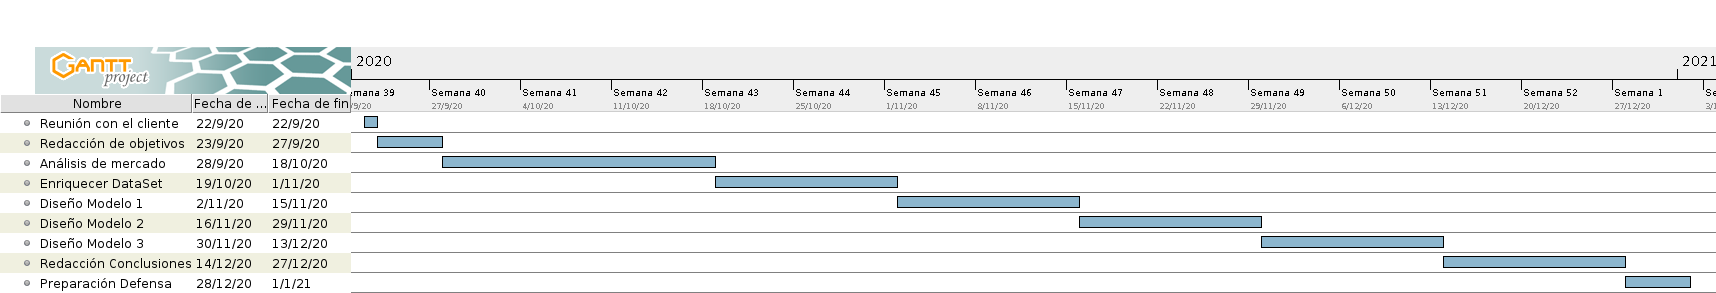
\includegraphics[width=0.9\textwidth]{figs/gant.png}
	\caption{Gantt del proyecto.}
	\label{fig:gant}
\end{figure}
\newpage
\section{Estado del arte}
\label{chapter:estado_del_arte}

\subsection{Recomendadores actuales}

\paragraph{}
A día de hoy, existen multitud de clasificadores y recomendadores\cite{ref:sorter_art_1} que se usan a diario para realizar todo tipo de recomendaciones, que van desde cual es el mejor producto en base a unas necesidades, pasando por clasificar piezas o productos en una fabrica para organizar la disponibilidad de estas, hasta incluso a recomendadores de canciones, series o películas en base a unas características de quien solicita estas.

\paragraph{}
Esto se ha conseguido gracias a la investigación y al IOT (Internet de las cosas 'Internet of Things') que facilita la vida a los investigadores y sobre todo a las personas. Antiguamente eran los usuarios los que, si querían comparar algo, tenían que buscar y buscar por tiendas para encontrar, o bien el mismo producto a distintos precios o bien productos alternativos al que quería adquirir o que directamente desconocía de la existencia de esa alternativa. Esto le consumía muchas horas (o incluso días) y ademas no tenia la garantía de haber abarcado todas las posibilidades\cite{ref:traditional_purchase_internet_purchase}.

\paragraph{}
Hoy en día, a través de Internet y gracias a los Recomendadores/Clasificadores actuales, el usuario puede consultar todas las alternativas y precios y estar mas seguro de que hace una buena elección antes de hacer la inversión\cite{ref:internet_comparatives}.

\paragraph{}
Los sistemas de recomendación/clasificación existen desde hace muchos años\cite{ref:history_recommender}. Han estado ahí para ayudarnos sin darnos cuenta, aunque al principio fueron muy rudimentarios. A medida que las características y el volumen de opciones crecía, se hacia más complicado y lento realizar esa clasificación/recomendación. Y en ese punto es donde entro los algoritmos de aprendizaje automático (\textit{Machine Learning}) para ayudar a que esas clasificaciones y recomendaciones fueran posibles en un tiempo razonable.

\paragraph{}
Dos empresas que quizás merezcan mención especial (gracias a la fama que consiguieron al implementar estos algoritmos) son \textit{Spotify}\cite{ref:music_recommender} con su recomendador de canciones y \textit{Netflix}\cite{ref:netflix} con su recomendador de series. Ambos utilizan el poder de los algoritmos de recomendadores de \textit{Machine Learning} para analizar el comportamiento que tienen sus usuarios en las correspondientes plataformas y sugerir recomendaciones basándose en estos comportamientos.


\subsection{Recomendadores en el ámbito de la medicina}
Pese a que en el ámbito de la medicina se ha utilizado mucho la estadística, el uso de estos recomendadores ha sido más discreto, o al menos no se ha dado a conocer su uso al publico potencial, llegando a quedarse en la fase de caso de estudio sin llegar a convertirse en un producto final. Un ejemplo de esto es el recomendador de medicamentos personalizado\cite{ref:refer_medical_prescriptions} que se basa en el historial clínico del paciente para recomendar la medicación que se ha de tomar este. Este es un caso de uso muy similar a nuestro \hyperref[op:OP1]{objetivo principal}, aunque en nuestro caso, buscamos recomendar referencias bibliográficas clínicas.

\paragraph{}
También se conocen casos donde se han usado estos Clasificadores/Recomendadores para clasificar muestras o grupos de individuos para realizar un posterior análisis del grupo, como por ejemplo este caso de uso\cite{ref:refer_classify_plaquetas} que utiliza un clasificador para clasificar plaquetas para un posterior ensayo medico.

\paragraph{}
Todo y con eso, como comentamos anteriormente, el uso de Clasificadores/Recomendadores en este ámbito suele pasar a estar en segundo plano por lo que se ha de intuir su uso para darse cuenta que sin ellos, muchos estudios no serian posibles a día de hoy.

\newpage
\subsection{Recomendadores en el ámbito de la salud}

\paragraph{}
Al igual que en el caso anterior, el uso de recomendadores en el ámbito de la salud pasa desapercibido y es raro la vez que se destaque como solución final para la ayuda a los profesionales sanitarios.

\paragraph{}
A continuación destacamos los más conocidos en este ámbito:

\paragraph{• Pubmed\cite{ref:pubmed_home}:}  Esta web Creada por el Centro Nacional de Biotecnología \textit{National Center for Biotechnology Information (NCBI)} Permite hacer búsquedas por texto libre y permite realizar filtros por año, tipo de artículo y disponibilidad del texto. En el listado también se puede observar el estado de los artículos, si la publicación es definitiva o aun se esta revisando su contenido. El orden de los resultados es por aproximación al texto que se busque (mejor acierto), aunque permite modificar la ordenación por fecha del artículo, nombre de autor u origen del artículo. En las figuras \ref{fig:pubmed1} y \ref{fig:pubmed2} puede ver el aspecto de la pagina y los resultados de una búsqueda.

\begin{figure}[h!]
    \begin{subfigure}[b]{0.45\linewidth}
    	\centering
		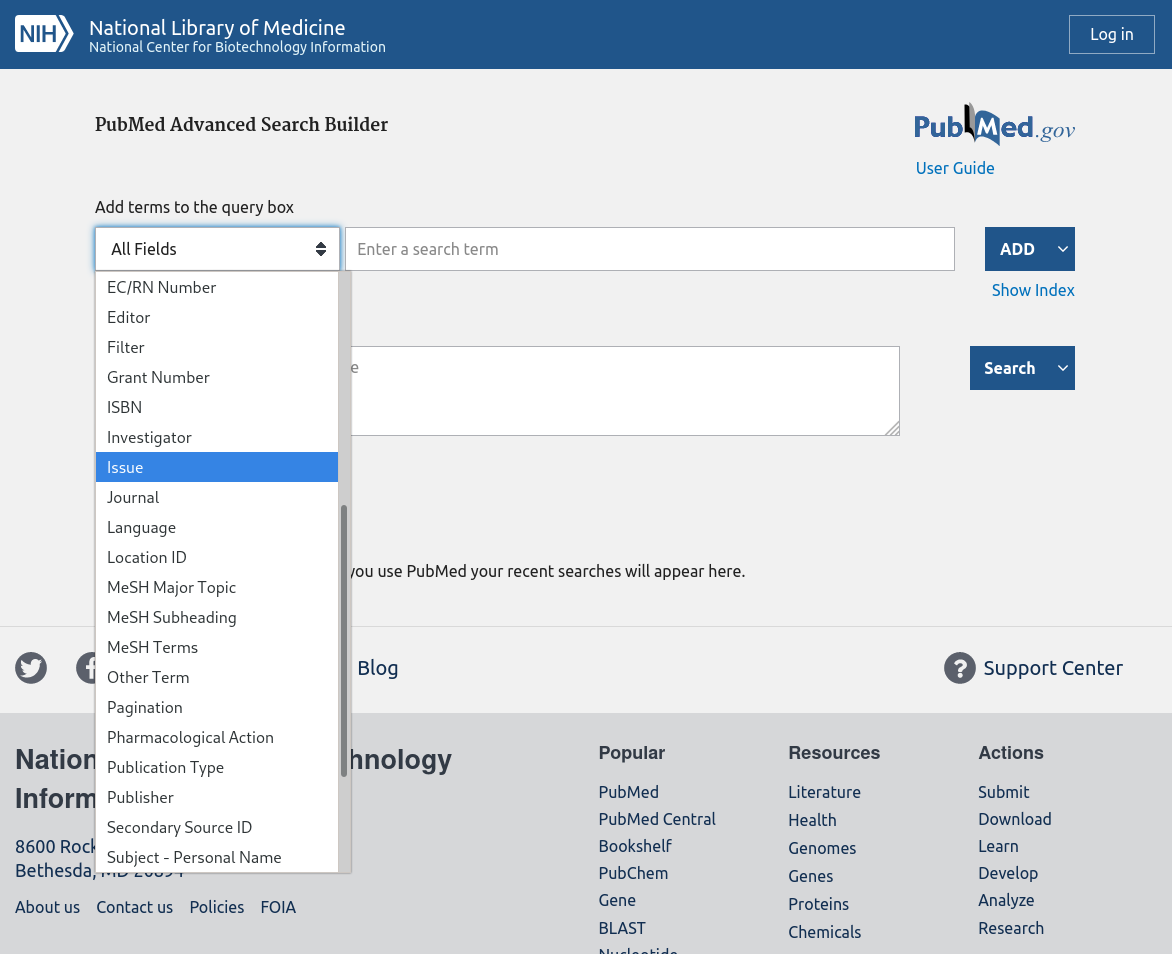
\includegraphics[width=0.9\textwidth]{images/Pubmed.png}
		\caption{Vista principal de Pubmed.}
		\label{fig:pubmed1}
	\end{subfigure}
	\begin{subfigure}[b]{0.45\linewidth} 
		\centering
		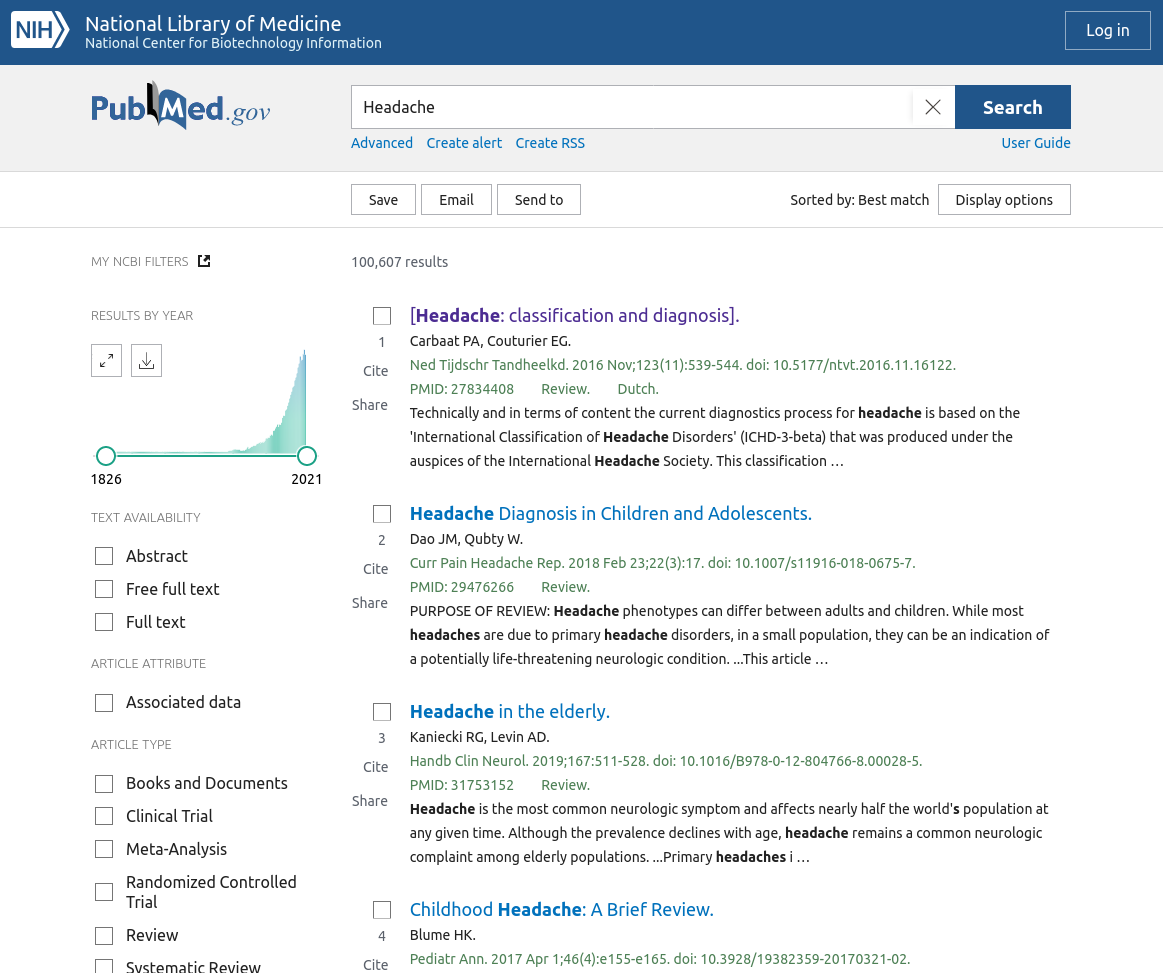
\includegraphics[width=0.9\textwidth]{images/Pubmed2.png}
		\caption{Resultados de búsqueda de Pubmed.}
		\label{fig:pubmed2}
	\end{subfigure}
	\caption{Web de Pubmed.}
	\label{fig:pubmed}
\end{figure}

\newpage
\paragraph{• ClinicalTrials\cite{ref:clinicaltrials_home}:} Esta web es una base de datos de estudios clínicos financiados con fondos públicos y privados realizados en todo el mundo. Permite realizar búsquedas y filtrados complejos de dolencias, mostrando los resultados en formato lista ordenados por fecha mas reciente, aunque el usuario puede elegir otras ordenaciones y filtrados. El listado también muestra el estado del documento (si ya esta finalizada la investigación o aun esta en proceso) y otra información relevante como el tratamiento que se esta aplicando. En las figuras \ref{fig:clinical_trials1} y \ref{fig:clinical_trials2} puede ver el aspecto de la pagina y los resultados de una búsqueda.

\begin{figure}[h!]
   	\centering
	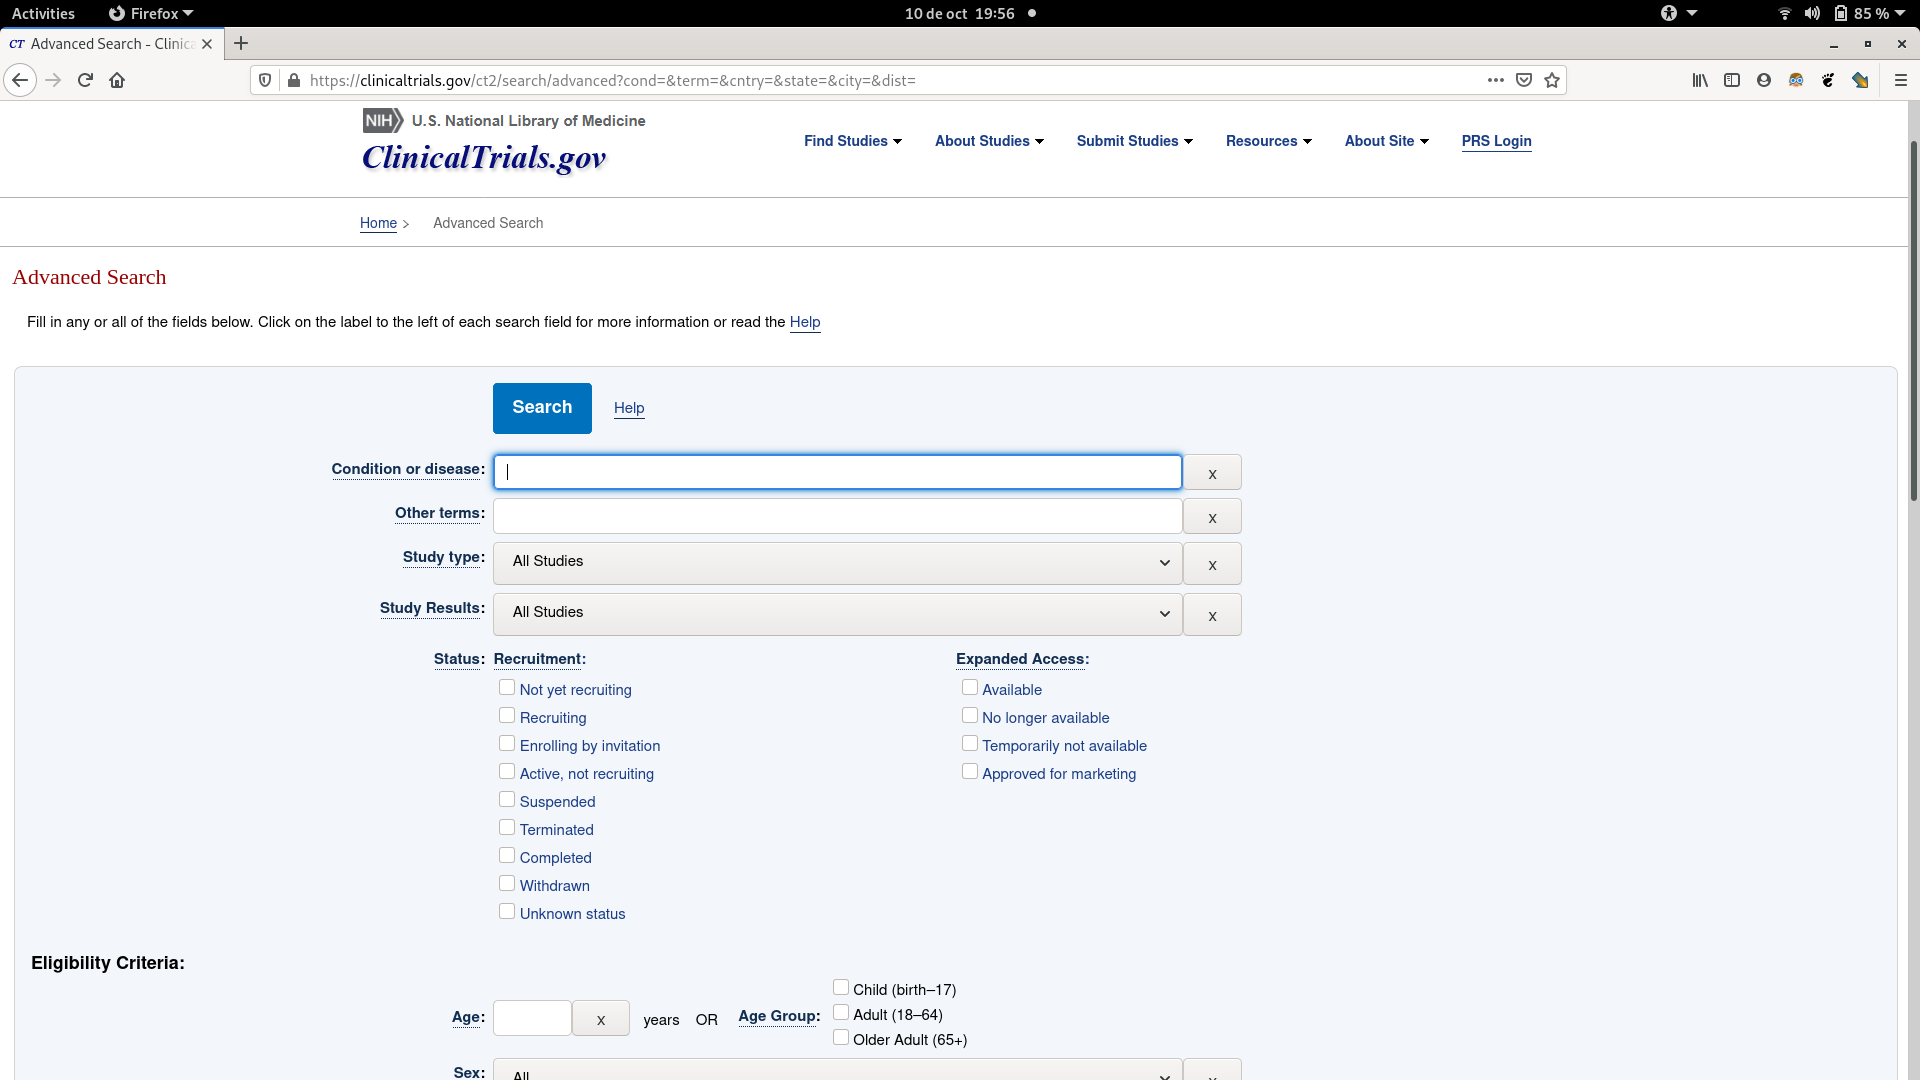
\includegraphics[width=0.7\textwidth]{images/ClinicalTrials.png}
	\caption{Vista principal de ClinicalTrials.}
	\label{fig:clinical_trials1}
\end{figure}

\begin{figure}[h!]
	\centering
	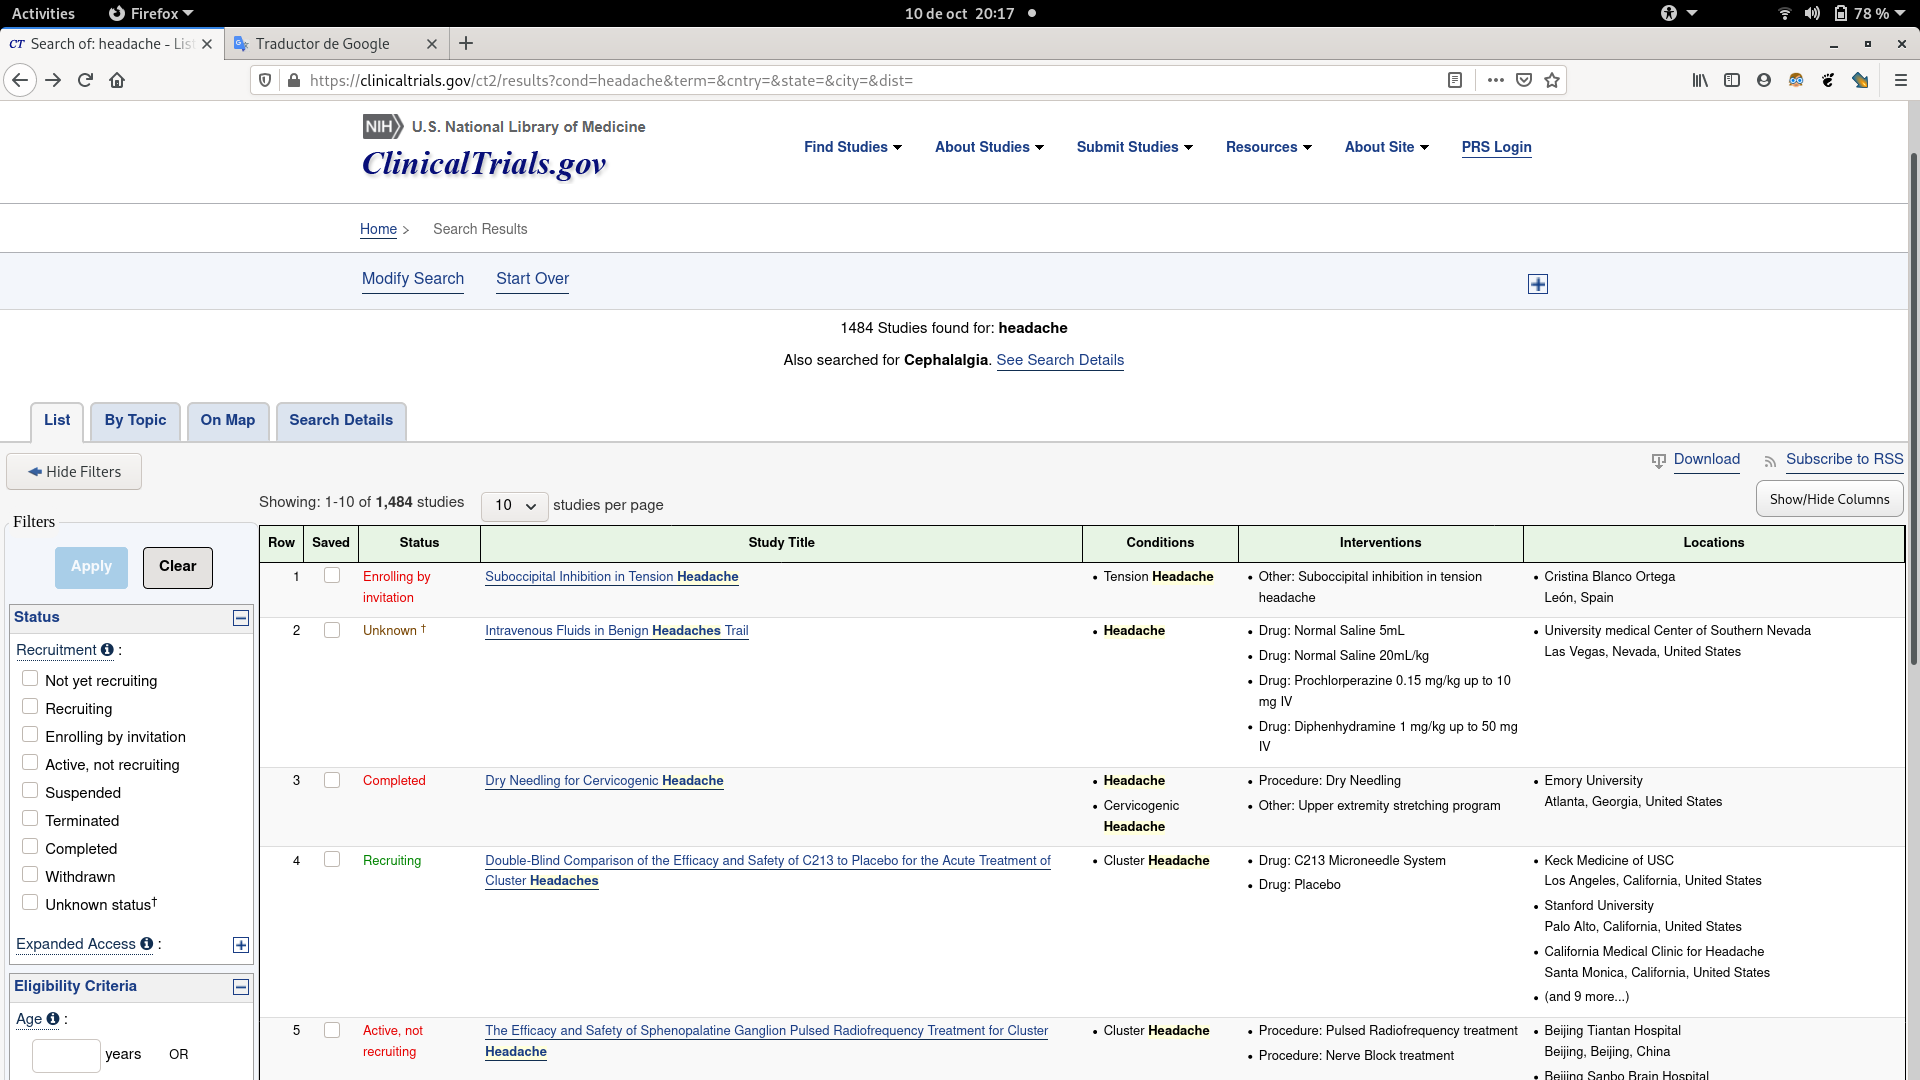
\includegraphics[width=0.7\textwidth]{images/ClinicalTrials2.png}
	\caption{Resultados de búsqueda de ClinicalTrials.}
	\label{fig:clinical_trials2}
\end{figure}

\newpage
\paragraph{• MedlinePlus\cite{ref:medlineplus_home}:} Esta web creada por Biblioteca Nacional de Medicina de EE. UU. (NLM, por sus siglas en inglés), esta más orientada al paciente que las anteriores, y permite buscar artículos médicos basándose en texto relacionado. Por ejemplo si ponemos un tipo de síntoma en el buscador, este nos muestra artículos relacionados con ese texto como si de un buscador de Internet común se tratara, aunque a diferencia de estos, MedlinePlus promete brindar información de calidad y relevante de salud y bienestar que sea confiable y fácil de entender. Aparentemente este buscador muestra los resultados en orden de relevancia aunque, igual que en los casos anteriores, no permite valorar si esos artículos son realmente interesantes para la búsqueda relacionada.En las figuras \ref{fig:medlineplus1} y \ref{fig:medlineplus2} puede ver el aspecto de la pagina y los resultados de una búsqueda.

\begin{figure}[h!]
    \begin{subfigure}[b]{0.45\linewidth}
    	\centering
		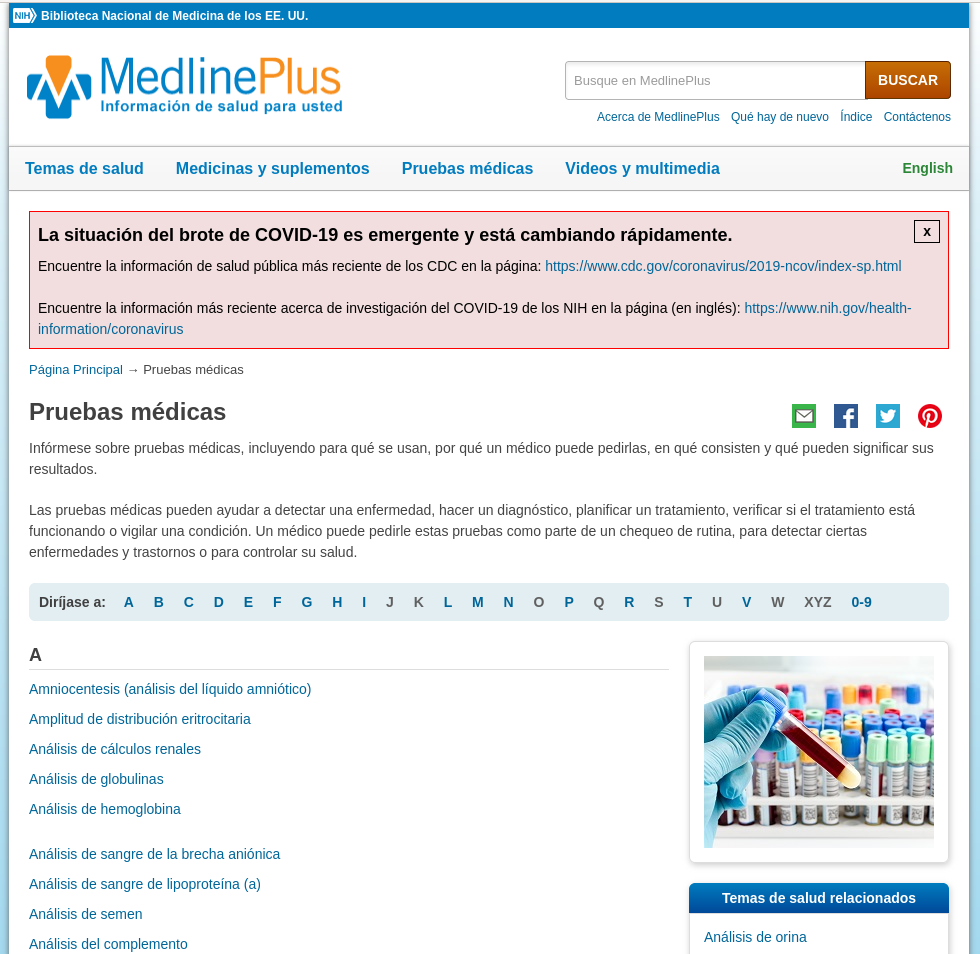
\includegraphics[width=0.9\textwidth]{images/MedlinePlus.png}
		\caption{Vista principal de MedlinePlus.}
		\label{fig:medlineplus1}
	\end{subfigure}
	\begin{subfigure}[b]{0.45\linewidth} 
		\centering
		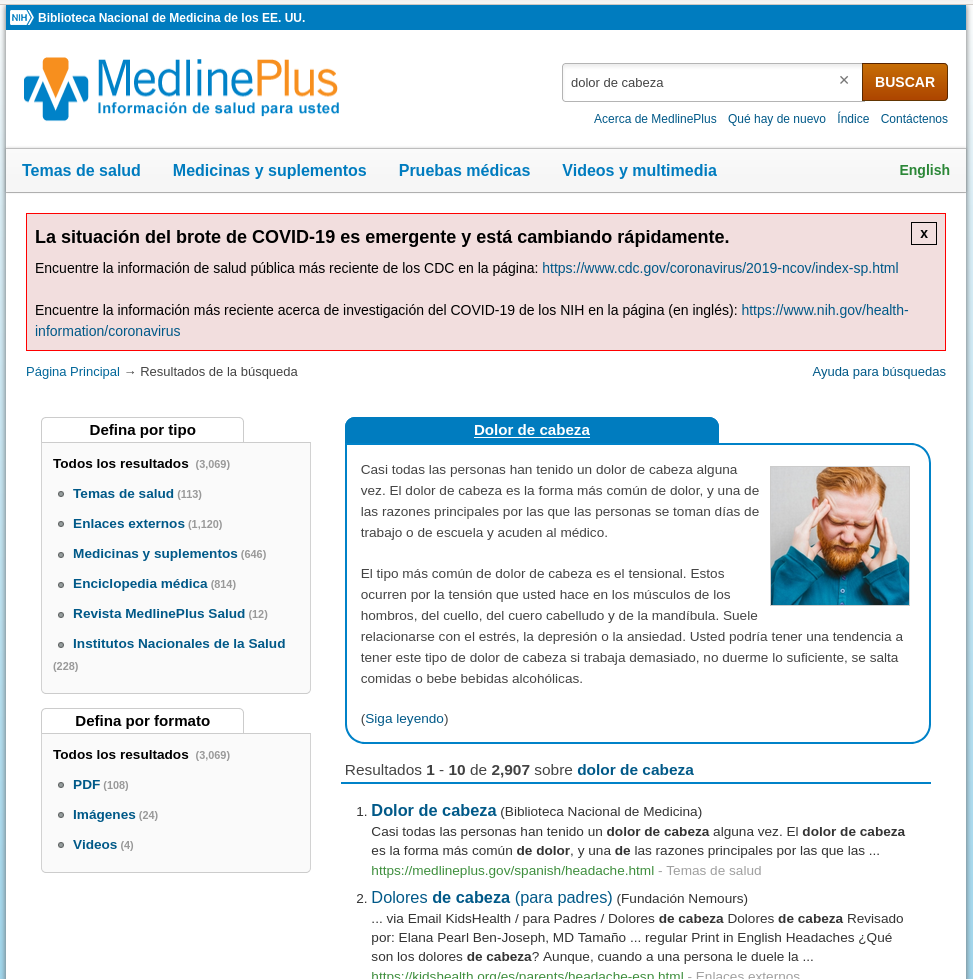
\includegraphics[width=0.9\textwidth]{images/MedlinePlus2.png}
		\caption{Resultados de búsqueda de MedlinePlus.}
		\label{fig:medlineplus2}
	\end{subfigure}
	\caption{Web de MedlinePlus.}
	\label{fig:medlineplus}
\end{figure}

\newpage
\subsection{Recomendadores en el futuro}

\paragraph{}
Los recomendadores/clasificadores han ayudado mucho en la medicina, sobre todo en el ámbito de la investigación, en donde se requiere un trabajo previo para poder tener un conjunto de datos valido para el posterior estudio que se quiera realizar. En el caso que nos toca, ayudará a los profesionales sanitarios a poder encontrar otras referencias bibliográficas personalizadas y adaptadas al estado del paciente, para así poder valorar alternativas. Este trabajo seria un trabajo eterno de realizar, por no decir casi imposible sin la ayuda de estos recomendadores/clasificadores, debido al gran volumen de información que cada día se genera. Estos algoritmos de recomendación/clasificación, no solo seguirán siendo un pilar básico en el ámbito medico, sino que seguramente aparecerán nuevos algoritmos de clasificación/recomendación que facilitaran las futuras investigaciones, como ya se esta observando en los nuevos recomendadores para el control de la glucosa en la sangre\cite{ref:refer_diabetes_control}.


\newpage

% bibliografia
\addcontentsline{toc}{chapter}{Bibliografía}
\bibliography{referencias}
\bibliographystyle{plain}


\end{document}